\chapter{La RMN en profundidad: pulsos, relajación y 2D}\label{ch:b3:advanced-nmr}

Un escáner de resonancia magnética de hospital y el espectrómetro de RMN de un departamento de química
funcionan con el mismo principio. Ambos colocan núcleos de hidrógeno en un campo magnético
intenso, inclinan su magnetización con un breve pulso de ondas de radio y
escuchan la débil señal que esta induce al precesar y relajarse. El
escáner convierte la señal en una imagen de los tejidos blandos; el espectrómetro, en
una lista de desplazamientos químicos y acoplamientos y, con varios pulsos seguidos,
en mapas bidimensionales que muestran qué átomo está enlazado a cuál. Este
capítulo explica qué hacen los pulsos, por qué se desvanece la señal y cómo se
leen los \omterm{def:b3:advanced-nmr:two-d}{espectros bidimensionales} ---el método con el que hoy se resuelven la mayoría de las nuevas
estructuras orgánicas.

\begin{recall}
El volumen del primer año interpretó espectros de RMN de ${}^1$H: desplazamiento químico, apantallamiento,
protones equivalentes, integración, acoplamiento espín--espín, constantes de acoplamiento y
multipletes. El volumen del segundo año añadió la RMN de ${}^{13}$C con desacoplamiento de banda ancha y
el DEPT, cuya secuencia de pulsos tomó como dada; los pulsos se explican aquí.
El \cref{ch:b3:many-electron-atoms} trató el espín como un momento angular. De la
física: un momento magnético en un campo tiene la energía $-\boldsymbol\mu\cdot\mathbf B$, y las
poblaciones de los niveles siguen el factor de Boltzmann $\eu^{-\Delta E/kT}$, desarrollado
en el \cref{ch:b3:partition-functions}.
\end{recall}

\begin{omfigure}
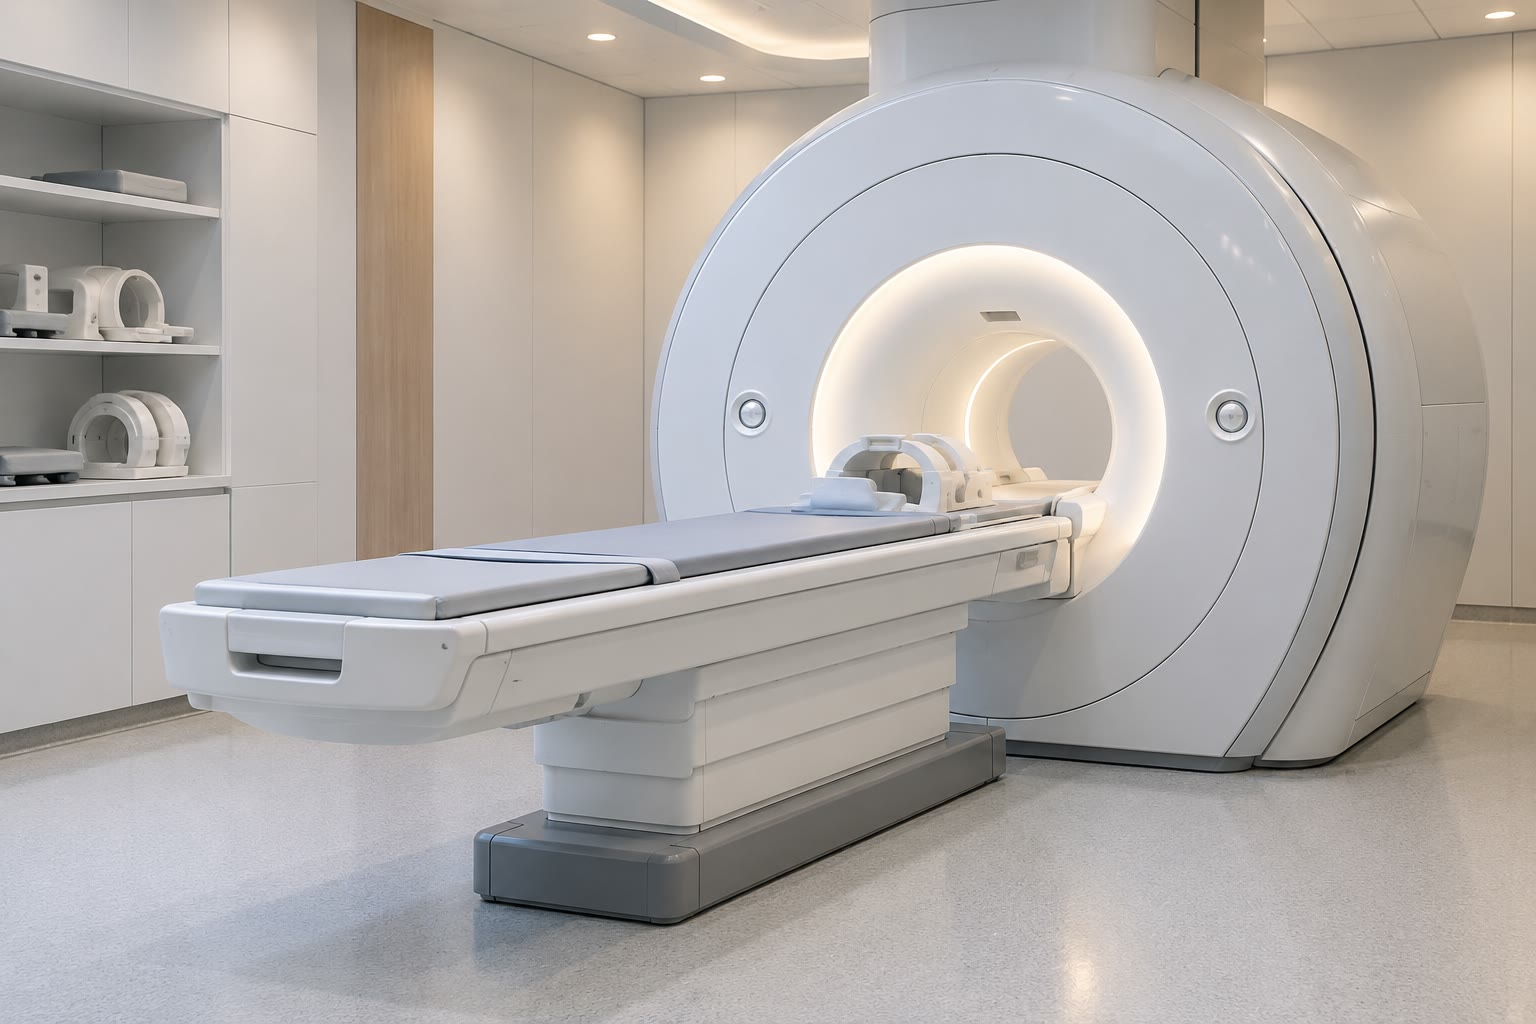
\includegraphics[width=0.52\linewidth]{images/book4/ai/b3-08-mri.jpg}\hspace{0.8em}%
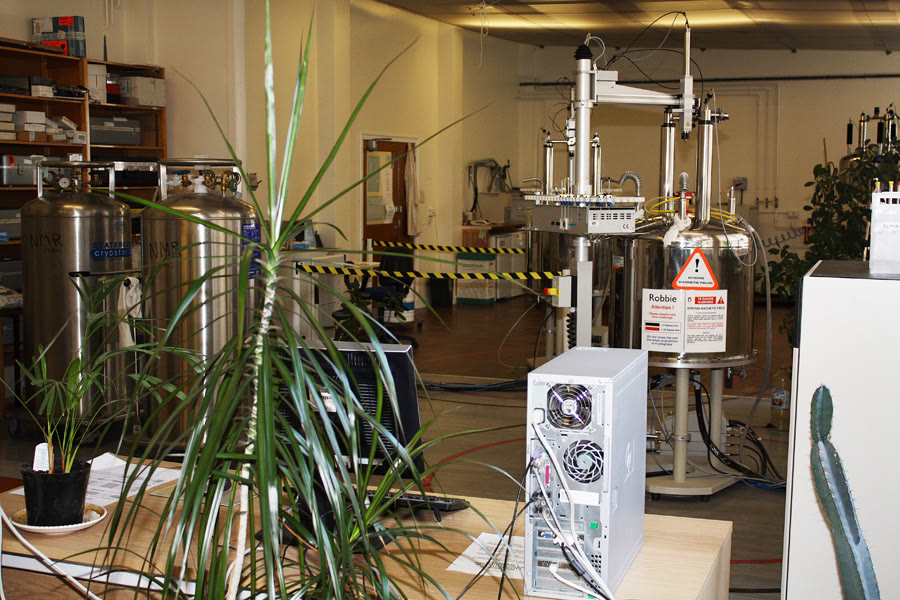
\includegraphics[width=0.4\linewidth]{images/book4/nmr-lab.jpg}

{\small Izquierda: un escáner de resonancia magnética de hospital. Derecha: un laboratorio de RMN; cada
imán superconductor está en su criostato, que se rellena con helio líquido
y nitrógeno líquido desde los dewars de la izquierda. Fotografía de Shandchem,
CC BY 2.0.}
\end{omfigure}

\section{Espines nucleares en un campo magnético}

\begin{definition}[Número cuántico de espín nuclear, relación giromagnética]\label{def:b3:advanced-nmr:nuclear-spin}
Un núcleo tiene un momento angular de espín de número cuántico $I$, su
\emph{número cuántico de espín nuclear}\index{numero cuantico de espin nuclear@número cuántico de espín nuclear} ($I = 0$
para \ce{^{12}C}, \ce{^{16}O}; $\frac12$ para \ce{^1H}, \ce{^{13}C}, \ce{^{15}N}, \ce{^{19}F},
\ce{^{31}P}; 1 para \ce{^2H}, \ce{^{14}N}), y un momento magnético $\boldsymbol\mu = \gamma\hat{\mathbf
I}$ proporcional a él; $\gamma$ es la \emph{relación giromagnética}\index{relacion giromagnetica@relación giromagnética}.
Según un campo $B_0$ (eje $z$), $\hat I_z$ toma los valores $m_I\hbar$,
$m_I = -I, \dots, I$.
\end{definition}

\begin{proposition}[Niveles Zeeman]\label{prop:b3:advanced-nmr:zeeman}
En un campo $B_0$, los niveles son $E_m = -m_I\gamma\hbar B_0$; las transiciones $\Delta m_I = \pm1$
absorben a la frecuencia
\[
\nu_0 = \frac{\gamma B_0}{2\pi}.
\]
\end{proposition}

\begin{proof}
$E = -\boldsymbol\mu\cdot\mathbf B = -\gamma B_0\hat I_z$, de \omterm{def:b3:quantum-model-systems:operator}{valores propios} $-\gamma B_0m_I\hbar$. Los niveles
adyacentes difieren en $\gamma\hbar B_0 = h\nu_0$.
\end{proof}

\begin{definition}[Frecuencia de Larmor]\label{def:b3:advanced-nmr:larmor}
$\nu_0 = \gamma B_0/2\pi$ es la \emph{frecuencia de Larmor}\index{frecuencia de Larmor} del
núcleo: la frecuencia de la resonancia, y también la frecuencia a la que su
momento magnético precesa en torno al campo.
\end{definition}

\begin{example}[Los núcleos habituales]\label{ex:b3:advanced-nmr:nuclei}
% ledger: const:gammaP, nuc:C13.mu, nuc:F19.mu, nuc:P31.mu, nuc:N15.mu, const:muN
Para un núcleo de espín $\frac12$ y momento $\mu$, $\gamma/2\pi = \mu/(Ih) = 2\mu/h$. Con los
momentos medidos: \ce{^1H} \qty{42.58}{MHz/T}, \ce{^{19}F} \qty{40.08}{MHz/T}, \ce{^{31}P}
\qty{17.25}{MHz/T}, \ce{^{13}C} \qty{10.71}{MHz/T}, \ce{^{15}N} \qty{-4.32}{MHz/T}. Un
``espectrómetro de \qty{400}{MHz}'' tiene $B_0 = \qty{9.4}{T}$: sus protones resuenan a
\qty{400.2}{MHz} y sus carbonos a \qty{100.7}{MHz}.
\end{example}

\begin{proposition}[Una diferencia de población minúscula]\label{prop:b3:advanced-nmr:populations}
Para un espín $\frac12$ a la temperatura $T$, el exceso de núcleos en el nivel inferior es
\[
\frac{N_\alpha - N_\beta}{N} \approx \frac{\gamma\hbar B_0}{2kT}.
\]
\end{proposition}

\begin{proof}
$N_\beta/N_\alpha = \eu^{-\Delta E/kT} \approx 1 - \Delta E/kT$, ya que $\Delta E \ll kT$; así,
$(N_\alpha - N_\beta)/(N_\alpha + N_\beta) \approx \Delta E/2kT$, con $\Delta E = \gamma\hbar B_0$.
\end{proof}

Para los protones a \qty{9.4}{T} y \qty{300}{K}, el exceso es de \num{3.2e-5}: solo
contribuyen tres núcleos de cada cien mil. Como tanto el exceso como la
tensión inducida en la bobina crecen con $\gamma$ y $B_0$, la señal crece
aproximadamente como $\gamma^3B_0^2$: de ahí la carrera hacia imanes cada vez más potentes, y la baja
sensibilidad de los núcleos con $\gamma$ pequeño y baja abundancia natural, como el
\ce{^{13}C}.

\section{Pulsos y decaimiento de inducción libre}

\begin{definition}[Magnetización neta, sistema de referencia rotatorio]\label{def:b3:advanced-nmr:magnetisation}
La \emph{magnetización neta}\index{magnetizacion neta@magnetización neta} $\mathbf M$ de una muestra es la
suma de sus momentos magnéticos nucleares por unidad de volumen; en el equilibrio vale
$M_0$ según $\mathbf B_0$. El \emph{sistema de referencia rotatorio}\index{sistema de referencia rotatorio} es un conjunto
de ejes $x'$, $y'$, $z$ que gira en torno a $z$ a la frecuencia de las ondas de radio
aplicadas; en él, la precesión a $\nu_0$ se ve frenada hasta la diferencia $\nu_0 -
\nu_{\mathrm{rf}}$.
\end{definition}

\begin{proposition}[Precesión]\label{prop:b3:advanced-nmr:precession}
Una magnetización en un campo obedece a $\dd\mathbf M/\dd t = \gamma\,\mathbf M\times\mathbf B$; en un
campo estático $B_0\mathbf e_z$, su componente transversal gira en torno a $z$ a la frecuencia
angular $\omega_0 = \gamma B_0$, mientras $M_z$ permanece constante.
\end{proposition}

\begin{proof}[Demostración parcial]
La ecuación es la ecuación clásica del momento de fuerza para un momento magnético que lleva
momento angular, que se admite de la física. Con $\mathbf B = B_0\mathbf e_z$: $\dot M_x = \gamma
B_0M_y$, $\dot M_y = -\gamma B_0M_x$, $\dot M_z = 0$, cuya solución es $M_x + \iu M_y \propto
\eu^{-\iu\gamma B_0t}$: una rotación a $\omega_0$ (en sentido horario vista desde $+z$ para $\gamma > 0$).
\end{proof}

\begin{definition}[Pulso de radiofrecuencia, ángulo de nutación]\label{def:b3:advanced-nmr:pulse}
Un \emph{pulso de radiofrecuencia}\index{pulso de radiofrecuencia} es una breve ráfaga de
ondas de radio a $\nu_{\mathrm{rf}} \approx \nu_0$, cuyo campo magnético $B_1$, fijo en el
sistema rotatorio según $x'$, hace girar $\mathbf M$ en torno a $x'$. El ángulo girado es el
\emph{ángulo de nutación}\index{angulo de nutacion@ángulo de nutación} $\theta = \gamma B_1t_p$ para un pulso de duración
$t_p$: un pulso de $90^\circ$ lleva $\mathbf M$ al plano $x'y'$, y uno de $180^\circ$ la
invierte.
\end{definition}

\begin{omfigure}
\tdplotsetmaincoords{70}{120}
\begin{tikzpicture}[tdplot_main_coords, font=\small, >=Stealth]
  \begin{scope}
    \draw[->, gray] (0,0,0) -- (1.8,0,0) node[anchor=north east] {$x'$};
    \draw[->, gray] (0,0,0) -- (0,1.8,0) node[anchor=north west] {$y'$};
    \draw[->, gray] (0,0,0) -- (0,0,1.8) node[anchor=south] {$z$, $\mathbf B_0$};
    \draw[->, omThm, very thick] (0,0,0) -- (0,0,1.4) node[anchor=west] {$\mathbf M$};
    \node[anchor=north] at (0,0,-0.9) {equilibrio};
  \end{scope}
  \begin{scope}[shift={(0,4.6,0)}]
    \draw[->, gray] (0,0,0) -- (1.8,0,0) node[anchor=north east] {$x'$};
    \draw[->, gray] (0,0,0) -- (0,1.8,0) node[anchor=north west] {$y'$};
    \draw[->, gray] (0,0,0) -- (0,0,1.8) node[anchor=south] {$z$};
    \draw[->, omDef, thick] (0,0,0) -- (1.2,0,0) node[anchor=south east, xshift=-2pt] {$\mathbf B_1$};
    \draw[->, omThm, very thick] (0,0,0) -- (0,1.4,0) node[anchor=south west] {$\mathbf M$};
    \node[anchor=north] at (0,0,-0.9) {tras un pulso $90^\circ_{x'}$};
  \end{scope}
  \begin{scope}[shift={(0,9.2,0)}]
    \draw[->, gray] (0,0,0) -- (1.8,0,0) node[anchor=north east] {$x'$};
    \draw[->, gray] (0,0,0) -- (0,1.8,0) node[anchor=north west] {$y'$};
    \draw[->, gray] (0,0,0) -- (0,0,1.8) node[anchor=south] {$z$};
    \draw[->, omThm, very thick] (0,0,0) -- (0,0,-1.4) node[anchor=west] {$\mathbf M$};
    \node[anchor=north] at (0,0,-1.6) {tras un pulso $180^\circ_{x'}$};
  \end{scope}
\end{tikzpicture}

{\small La magnetización en el \omterm{def:b3:advanced-nmr:magnetisation}{sistema de referencia rotatorio}. Un pulso de $90^\circ$ en torno a $x'$
lleva $\mathbf M$ de $z$ a $y'$ (con $\gamma > 0$, la rotación sigue la regla de la
mano izquierda en torno a $\mathbf B_1$, el convenio habitual); un pulso de $180^\circ$
la invierte.}
\end{omfigure}

\begin{definition}[Decaimiento de inducción libre]\label{def:b3:advanced-nmr:fid}
Tras un pulso de $90^\circ$, la magnetización transversal precesa a la \omterm{def:b3:advanced-nmr:larmor}{frecuencia de
Larmor} e induce una tensión oscilante en la bobina que rodea la muestra,
que se extingue a medida que la magnetización se relaja: es el \emph{decaimiento de inducción
libre}\index{decaimiento de induccion libre@decaimiento de inducción libre} (FID).
\end{definition}

\begin{theorem}[Del FID al espectro]\label{thm:b3:advanced-nmr:lorentzian}
La transformada de Fourier de una oscilación amortiguada $\eu^{-t/T_2}\cos(2\pi\nu t)$ ($t \ge 0$) es,
cerca de $\nu$, una raya lorentziana de anchura total a media altura $1/(\pi T_2)$.
\end{theorem}

\begin{proof}
Si se escribe la señal como $\eu^{-t/T_2}\eu^{2\pi\iu\nu t}$ y se integra, se obtiene
$\int_0^\infty\eu^{-t/T_2}\eu^{2\pi\iu(\nu - f)t}\dd t = \frac{1}{1/T_2 - 2\pi\iu(\nu - f)}$, cuya
parte real es $\frac{T_2}{1 + 4\pi^2T_2^2(f - \nu)^2}$. Es máxima en $f = \nu$ y cae a
la mitad cuando $2\pi T_2|f - \nu| = 1$, es decir, en $f - \nu = \pm1/(2\pi T_2)$: una anchura
total de $1/(\pi T_2)$.
\end{proof}

\begin{omfigure}
\begin{tikzpicture}
\begin{axis}[name=fid, width=0.5\linewidth, height=4.6cm, xmin=0, xmax=0.4,
  ymin=-2.1, ymax=2.1, axis lines=left, xlabel={$t$ / s}, ylabel={señal},
  ytick=\empty, scaled x ticks=false, xticklabel style={/pgf/number format/fixed},
  tick label style={font=\small}, label style={font=\small}, title={\small FID}]
\addplot[omDef] table[x=t, y=s] {figdata/out/bachelor-3-nmr-fid.dat};
\addplot[gray, dashed, domain=0:0.4, samples=60] {2*exp(-x/0.1)};
\end{axis}
\begin{axis}[at={(fid.east)}, anchor=west, xshift=1.2cm, width=0.45\linewidth,
  height=4.6cm, xmin=0, xmax=350, ymin=-0.1, ymax=1.1, axis x line=bottom,
  axis y line=none, xlabel={diferencia / Hz}, tick label style={font=\small},
  label style={font=\small}, title={\small espectro (transformada de Fourier)}]
\addplot[omThm, thick] table[x=f, y=I] {figdata/out/bachelor-3-nmr-fid-spectrum.dat};
\end{axis}
\end{tikzpicture}

{\small Izquierda: el FID de dos rayas (diferencias de 100 y \qty{250}{Hz}, $T_2 = \qty{0.10}{s}$),
con pulsaciones por la interferencia de las dos frecuencias dentro de una envolvente exponencial
(trazo discontinuo). Derecha: su transformada de Fourier, dos rayas lorentzianas de \qty{3.2}{Hz} de anchura.}
\end{omfigure}

\begin{proposition}[Acumulación de señal]\label{prop:b3:advanced-nmr:averaging}
Sumar $N$ FID multiplica la señal por $N$ y el ruido aleatorio por $\sqrt N$:
la relación señal/ruido crece como $\sqrt N$.
\end{proposition}

\begin{proof}
La señal se suma de forma coherente. El ruido de adquisiciones independientes tiene
media nula y varianza $\sigma^2$ cada una; la varianza de una suma de $N$ términos independientes es
$N\sigma^2$ (la ley de propagación del volumen del segundo año), de modo que su desviación típica
es $\sqrt N\sigma$.
\end{proof}

El DEPT, que clasifica las señales de ${}^{13}$C según el número de hidrógenos unidos,
aplica una secuencia de pulsos a protones y carbonos separados por
esperas de $1/2J$: la gran magnetización de los protones se transfiere al carbono
a través del acoplamiento a un enlace, lo que multiplica la señal del carbono por unos
$\gamma_H/\gamma_C \approx 4$, y el ángulo del último pulso de protones pondera de distinto modo CH, \ce{CH2} y
\ce{CH3}. La misma idea ---trasladar magnetización entre núcleos
a través de sus acoplamientos--- está en la base de los experimentos bidimensionales que siguen.

\section{Relajación}

\begin{definition}[Tiempos de relajación longitudinal y transversal]\label{def:b3:advanced-nmr:relaxation}
El retorno de $M_z$ a $M_0$ tras una perturbación es exponencial, con el
\emph{tiempo de relajación longitudinal}\index{tiempo de relajacion longitudinal@tiempo de relajación longitudinal} $T_1$
(relajación espín--red: energía cedida al entorno). El decaimiento de
la magnetización transversal hasta cero es exponencial, con el
\emph{tiempo de relajación transversal}\index{tiempo de relajacion transversal@tiempo de relajación transversal} $T_2 \le T_1$
(relajación espín--espín: pérdida de coherencia de fase entre los espines).
\end{definition}

\begin{proposition}[Inversión-recuperación]\label{prop:b3:advanced-nmr:inversion-recovery}
Tras un pulso de $180^\circ$, $M_z(t) = M_0(1 - 2\eu^{-t/T_1})$; pasa por cero en
$t_{\mathrm{nulo}} = T_1\ln2$.
\end{proposition}

\begin{proof}
La ecuación de relajación $\dd M_z/\dd t = (M_0 - M_z)/T_1$ con $M_z(0) = -M_0$ tiene la
solución $M_0 - 2M_0\eu^{-t/T_1}$, que se anula cuando $\eu^{-t/T_1} = \frac12$.
\end{proof}

\begin{method}[Medir $T_1$ y fijar una espera de reciclado cuantitativa]\label{met:b3:advanced-nmr:t1}
\begin{enumerate}
  \item Ejecutar la secuencia $180^\circ$--$\tau$--$90^\circ$--adquisición para una serie de esperas
        $\tau$, aguardando al menos $5T_1$ entre barridos.
  \item Ajustar cada señal a $M_0(1 - 2\eu^{-\tau/T_1})$, o leer el paso por cero: $T_1 =
        t_{\mathrm{nulo}}/\ln2$.
  \item Para una integración cuantitativa con pulsos de $90^\circ$, esperar al menos $5T_1$ del
        núcleo más lento entre barridos: así falta $\eu^{-5} < 1\,\%$ de la
        magnetización.
\end{enumerate}
\end{method}

\begin{omfigure}
\begin{tikzpicture}
\begin{axis}[width=0.62\linewidth, height=5cm, xmin=0, xmax=10, ymin=-1.1, ymax=1.15,
  axis lines=left, xlabel={$t$ / s}, ylabel={$M/M_0$}, legend cell align=left,
  legend style={font=\small, draw=none, at={(0.97,0.05)}, anchor=south east},
  tick label style={font=\small}, label style={font=\small}]
\addplot[omDef, thick] table[x=t, y=mz] {figdata/out/bachelor-3-nmr-relaxation.dat};
\addlegendentry{$M_z$ tras $180^\circ$ ($T_1 = \qty{2.0}{s}$)}
\addplot[omThm, thick, dashed] table[x=t, y=mxy] {figdata/out/bachelor-3-nmr-relaxation.dat};
\addlegendentry{$M_{xy}$ tras $90^\circ$ ($T_2 = \qty{0.5}{s}$)}
\addplot[gray, dotted, domain=0:10] {0};
\addplot[only marks, mark=*, mark size=1.5pt, black] coordinates {(1.386,0)};
\node[font=\small, anchor=north west] at (axis cs:1.5,-0.04) {$T_1\ln2$};
\end{axis}
\end{tikzpicture}

{\small Relajación (valores modelo). La magnetización longitudinal invertida
se recupera pasando por cero en $T_1\ln2$; la magnetización transversal decae
más deprisa, con $T_2$.}
\end{omfigure}

\begin{definition}[Eco de espín]\label{def:b3:advanced-nmr:echo}
En la secuencia $90^\circ$--$\tau$--$180^\circ$--$\tau$, los espines que se han desfasado
por las inhomogeneidades del campo se reenfocan en el instante $2\tau$ y producen un
\emph{eco de espín}\index{eco de espin@eco de espín}; su amplitud decae con el verdadero $T_2$, libre de
la inhomogeneidad del imán.
\end{definition}

\begin{definition}[Efecto Overhauser nuclear]\label{def:b3:advanced-nmr:noe}
Saturar o perturbar un espín cambia, a través de su relajación
dipolar, la intensidad de la señal de otro espín próximo en el espacio:
es el \emph{efecto Overhauser nuclear}\index{efecto Overhauser nuclear} (NOE).
Su velocidad de crecimiento es proporcional a $r^{-6}$, de modo que solo se observa entre
núcleos separados menos de unos \qty{0.5}{nm}, estén enlazados o no.
\end{definition}

\section{RMN bidimensional}

\begin{definition}[Espectro bidimensional, pico de cruce, pico diagonal]\label{def:b3:advanced-nmr:two-d}
Un \emph{espectro bidimensional}\index{espectro bidimensional} se registra
repitiendo una secuencia de pulsos con una espera $t_1$, que se va incrementando, antes del
tiempo de adquisición $t_2$; una doble transformada de Fourier da un mapa de intensidad
en función de dos frecuencias. Un \emph{pico de cruce}\index{pico de cruce} en $(\delta_1,
\delta_2)$ muestra que los núcleos a $\delta_1$ y $\delta_2$ están conectados (por un acoplamiento o
por proximidad); un \emph{pico diagonal}\index{pico diagonal} en $(\delta, \delta)$ pertenece a
un solo núcleo.
\end{definition}

\begin{definition}[COSY, HSQC, HMBC, NOESY]\label{def:b3:advanced-nmr:experiments}
El \emph{COSY}\index{COSY} (espectroscopia de correlación) correlaciona protones acoplados
entre sí, normalmente a través de tres enlaces (H--C--C--H). El \emph{HSQC}\index{HSQC}
(coherencia heteronuclear de cuanto único) correlaciona cada carbono con los
protones directamente unidos a él. El \emph{HMBC}\index{HMBC} (correlación heteronuclear
a varios enlaces) correlaciona carbonos con protones situados a dos o tres enlaces,
a través de carbonos cuaternarios y heteroátomos. El \emph{NOESY}\index{NOESY}
correlaciona protones próximos en el espacio a través del \omterm{def:b3:advanced-nmr:noe}{efecto Overhauser nuclear}.
\end{definition}

\begin{omfigure}
\begin{tikzpicture}[font=\small]
  \foreach \y/\name in {3.2/{un pulso}, 2.0/{inversión-recuperación}, 0.8/{eco de espín}, -0.4/{COSY}}{
    \draw (0,\y) -- (9.3,\y); \node[anchor=east] at (-0.1,\y+0.25) {\name};}
  % one pulse
  \fill[black] (0.4,3.2) rectangle (0.6,3.75);
  \draw[omDef, domain=0:3.5, samples=120] plot (0.7+\x, {3.2+0.4*exp(-\x/1.2)*sin(\x*500)});
  % inversion recovery
  \fill[black] (0.4,2.0) rectangle (0.8,2.55); \node[font=\scriptsize] at (0.6,2.7) {180};
  \draw[<->] (0.85,1.85) -- (2.4,1.85) node[midway, below, font=\scriptsize] {$\tau$};
  \fill[black] (2.45,2.0) rectangle (2.65,2.55); \node[font=\scriptsize] at (2.55,2.7) {90};
  \draw[omDef, domain=0:3.0, samples=120] plot (2.75+\x, {2.0+0.4*exp(-\x/1.0)*sin(\x*500)});
  % spin echo
  \fill[black] (0.4,0.8) rectangle (0.6,1.35); \node[font=\scriptsize] at (0.5,1.5) {90};
  \draw[<->] (0.65,0.65) -- (2.4,0.65) node[midway, below, font=\scriptsize] {$\tau$};
  \fill[black] (2.45,0.8) rectangle (2.85,1.35); \node[font=\scriptsize] at (2.65,1.5) {180};
  \draw[<->] (2.9,0.65) -- (4.65,0.65) node[midway, below, font=\scriptsize] {$\tau$};
  \draw[omDef, domain=-1.2:2.5, samples=150] plot (4.65+\x, {0.8+0.35*exp(-abs(\x)/0.35)*cos(\x*700)});
  % COSY
  \fill[black] (0.4,-0.4) rectangle (0.6,0.15); \node[font=\scriptsize] at (0.5,0.3) {90};
  \draw[<->] (0.65,-0.55) -- (2.4,-0.55) node[midway, below, font=\scriptsize] {$t_1$ (incrementado)};
  \fill[black] (2.45,-0.4) rectangle (2.65,0.15); \node[font=\scriptsize] at (2.55,0.3) {90};
  \draw[omDef, domain=0:3.0, samples=120] plot (2.75+\x, {-0.4+0.4*exp(-\x/1.0)*sin(\x*500)});
  \node[font=\scriptsize, anchor=west] at (5.9,-0.2) {adquisición ($t_2$)};
\end{tikzpicture}

{\small Secuencias de pulsos (el tiempo avanza hacia la derecha; rectángulos llenos: pulsos, etiquetados
con su \omterm{def:b3:advanced-nmr:pulse}{ángulo de nutación} en grados; en azul, la señal registrada). El \omterm{def:b3:advanced-nmr:echo}{eco de espín}
alcanza su máximo a $2\tau$ del primer pulso.}
\end{omfigure}

\begin{method}[Resolver una estructura con espectros bidimensionales]\label{met:b3:advanced-nmr:solve-2d}
\begin{enumerate}
  \item A partir de la fórmula, de las integrales de ${}^1$H y del espectro de ${}^{13}$C/DEPT, enumerar
        los carbonos CH, \ce{CH2}, \ce{CH3} y cuaternarios.
  \item \omterm{def:b3:advanced-nmr:experiments}{HSQC}: asignar cada señal de protón a su carbono.
  \item \omterm{def:b3:advanced-nmr:experiments}{COSY}: unir los carbonos protonados en sistemas de espín (cadenas de
        vecinos).
  \item \omterm{def:b3:advanced-nmr:experiments}{HMBC}: unir los sistemas de espín a través de carbonos cuaternarios, carbonilos y
        heteroátomos, donde el \omterm{def:b3:advanced-nmr:experiments}{COSY} no dice nada.
  \item \omterm{def:b3:advanced-nmr:experiments}{NOESY}: fijar configuraciones relativas y conformaciones a partir de los
        contactos a través del espacio.
  \item Comprobar cada señal con la estructura propuesta.
\end{enumerate}
\end{method}

\begin{omfigure}
\begin{tikzpicture}
\begin{axis}[name=cosy, width=0.47\linewidth, height=0.47\linewidth, x dir=reverse,
  y dir=reverse, xmin=0.5, xmax=4.6, ymin=0.5, ymax=4.6, axis lines=box,
  xlabel={$\delta_{\mathrm H}$ / ppm}, ylabel={$\delta_{\mathrm H}$ / ppm},
  tick label style={font=\small}, label style={font=\small}, title={\small COSY}]
\addplot[gray, dotted, domain=0.5:4.6] {x};
\addplot[only marks, mark=*, mark size=2.2pt, black] table[x=h1, y=h2] {figdata/out/bachelor-3-nmr-2d-cosy-diag.dat};
\addplot[only marks, mark=*, mark size=2.2pt, omThm] table[x=h1, y=h2] {figdata/out/bachelor-3-nmr-2d-cosy-cross.dat};
\end{axis}
\begin{axis}[at={(cosy.east)}, anchor=west, xshift=1.3cm, width=0.47\linewidth,
  height=0.47\linewidth, x dir=reverse, y dir=reverse, xmin=0.5, xmax=4.6,
  ymin=0, ymax=185, axis lines=box, xlabel={$\delta_{\mathrm H}$ / ppm},
  ylabel={$\delta_{\mathrm C}$ / ppm}, tick label style={font=\small},
  label style={font=\small}, title={\small HSQC (azul) y HMBC (rojo)}]
\addplot[only marks, mark=square*, mark size=2.2pt, omDef] table[x=h, y=c] {figdata/out/bachelor-3-nmr-2d-hsqc.dat};
\addplot[only marks, mark=o, mark size=2.6pt, omThm, thick] table[x=h, y=c] {figdata/out/bachelor-3-nmr-2d-hmbc.dat};
\end{axis}
\end{tikzpicture}

{\small \omterm{def:b3:advanced-nmr:two-d}{Espectros bidimensionales} del butanoato de etilo, \ce{CH3CH2CH2COOCH2CH3},
dibujados con sus desplazamientos medidos. \omterm{def:b3:advanced-nmr:experiments}{COSY}: en negro, los \omterm{def:b3:advanced-nmr:two-d}{picos diagonales}; en rojo, los \omterm{def:b3:advanced-nmr:two-d}{picos de cruce}
entre protones de carbonos vecinos ---dos sistemas de espín, etilo y
propilo, sin ningún \omterm{def:b3:advanced-nmr:two-d}{pico de cruce} a través del oxígeno del éster. Derecha: los picos \omterm{def:b3:advanced-nmr:experiments}{HSQC}
(cuadrados) unen cada protón con su carbono; los picos \omterm{def:b3:advanced-nmr:experiments}{HMBC} (círculos) muestran que los protones
OCH$_2$ (\qty{4.13}{ppm}) y los protones CH$_2$C=O (\qty{2.28}{ppm}) alcanzan ambos el
carbono carbonílico a \qty{173.6}{ppm}.}
\end{omfigure}

\section{Otros núcleos y dinámica}

El flúor 19 y el fósforo 31, de espín $\frac12$, abundantes al 100\,\% y con $\gamma$
grande, son casi tan fáciles de observar como los protones; sus amplios intervalos de desplazamientos los convierten
en sondas precisas de su entorno (fármacos, fosfatos, ligandos como las
fosfinas del \cref{ch:b3:organometallic-bonding}). El nitrógeno 15 es raro y
débil, y suele observarse indirectamente a través de los protones unidos a él.
El acoplamiento entre núcleos distintos se elimina por desacoplamiento, como para el ${}^{13}$C en
el volumen del segundo año.

\begin{definition}[Temperatura de coalescencia]\label{def:b3:advanced-nmr:coalescence}
Cuando un núcleo se intercambia entre dos entornos de desplazamientos separados por
$\Delta\nu$ (en hercios), sus dos rayas se ensanchan a medida que el intercambio se acelera y se funden
en una sola a la \emph{temperatura de coalescencia}\index{temperatura de coalescencia}
$T_c$.
\end{definition}

\begin{proposition}[Velocidad en la coalescencia]\label{prop:b3:advanced-nmr:coalescence}
Para dos sitios igualmente poblados sin acoplamiento, la constante de velocidad de intercambio en
la coalescencia es $k_c = \pi\Delta\nu/\sqrt2$.
\end{proposition}
\admitted

La deducción, a partir de las ecuaciones de Bloch con intercambio, corresponde a cursos más
avanzados. Con la ecuación de Eyring (\cref{ch:b3:rate-theories}), la velocidad
da la barrera: la RMN dinámica mide rotaciones en torno a enlaces amida, inversiones de
anillos e intercambios de ligandos con barreras de 40 a \qty{100}{kJ/mol}.

\begin{example}[Una imagen de resonancia magnética]\label{ex:b3:advanced-nmr:mri}
En la resonancia magnética de imagen, un gradiente de campo hace que la \omterm{def:b3:advanced-nmr:larmor}{frecuencia de Larmor} de
los protones del agua dependa de la posición, de modo que la transformada de Fourier de la
señal es un mapa de dónde están. El contraste procede de la relajación: el
tiempo de repetición y las esperas de eco se eligen para ponderar la imagen por $T_1$ o por
$T_2$, que difieren de un tejido a otro; los agentes de contraste que contienen gadolinio
acortan el $T_1$ del agua cercana (\cref{ch:b3:bioinorganic}).
\end{example}

\begin{inthelab}[Preparar un espectrómetro]
La muestra, disuelta en un disolvente deuterado, se baja hasta la sonda.
El espectrómetro se enclava (``lock'') en la señal del deuterio para compensar la lenta deriva del
campo; la sonda se sintoniza y se adapta a la frecuencia de cada núcleo;
el campo se hace homogéneo sobre la muestra ajustando las bobinas de corrección (``shims'')
hasta que las rayas son estrechas. El campo del imán es permanente: las herramientas de acero,
las tarjetas de crédito y los marcapasos se mantienen fuera de la línea de seguridad marcada.
\end{inthelab}

\begin{history}[De la resonancia a las dos dimensiones]
Felix Bloch y Edward Purcell detectaron la resonancia magnética nuclear en la materia
condensada en 1946 (premio Nobel de Física, 1952). Richard Ernst introdujo la RMN pulsada
por transformada de Fourier en 1966 y, siguiendo una idea de Jean Jeener,
la espectroscopia bidimensional en la década de 1970 (premio Nobel de Química, 1991).
\end{history}

\section{Ejercicios}

\begin{exercise}[$\star$]\label{exo:b3:advanced-nmr:1}
% ledger: const:gammaP, nuc:C13.mu, nuc:F19.mu
Calcúlense las \omterm{def:b3:advanced-nmr:larmor}{frecuencias de Larmor} de \ce{^1H}, \ce{^{13}C} y \ce{^{19}F} a \qty{14.1}{T}
($\gamma/2\pi = 42.58$, 10.71 y \qty{40.08}{MHz/T}).
\end{exercise}

\begin{exercise}[$\star$]\label{exo:b3:advanced-nmr:2}
Calcúlese el exceso relativo de protones en el nivel inferior a \qty{9.4}{T} y
\qty{300}{K}. ¿Cuánto cambia a \qty{4}{K}?
\end{exercise}

\begin{exercise}[$\star$]\label{exo:b3:advanced-nmr:3}
Un pulso de $90^\circ$ dura \qty{10}{\micro s} para los protones. ¿Cuánto vale $\gamma B_1/2\pi$? ¿Cuánto dura un
pulso de $180^\circ$, y qué hace un pulso de \qty{5}{\micro s}?
\end{exercise}

\begin{exercise}[$\star$]\label{exo:b3:advanced-nmr:4}
Una raya tiene \qty{3.2}{Hz} de anchura a media altura. ¿Cuánto vale $T_2$ (suponiendo un campo
perfectamente homogéneo)?
\end{exercise}

\begin{exercise}[$\star\star$]\label{exo:b3:advanced-nmr:5}
% ledger: iso:C13
Usando una señal $\propto\gamma^3$ por núcleo y la abundancia natural del 1.1\,\% del
\ce{^{13}C}, compárese la sensibilidad de la RMN de ${}^{13}$C y de ${}^1$H. ¿Cuántos barridos más
necesita un espectro de ${}^{13}$C para la misma relación señal/ruido?
\end{exercise}

\begin{exercise}[$\star\star$]\label{exo:b3:advanced-nmr:6}
En un experimento de inversión-recuperación, la señal de un carbono se anula en
$\tau = \qty{1.39}{s}$. Encuéntrense $T_1$ y la espera de reciclado para un trabajo cuantitativo.
\end{exercise}

\begin{exercise}[$\star\star$]\label{exo:b3:advanced-nmr:7}
En el espectro \omterm{def:b3:advanced-nmr:experiments}{COSY} de la butanona, \ce{CH3COCH2CH3}, ¿qué \omterm{def:b3:advanced-nmr:two-d}{picos de cruce} aparecen?
¿Qué carbonos presentan picos \omterm{def:b3:advanced-nmr:experiments}{HMBC} procedentes de los protones del metilo singlete?
\end{exercise}

\begin{exercise}[$\star\star$]\label{exo:b3:advanced-nmr:8}
Dos señales de metilo de una amida, separadas \qty{50}{Hz} a baja temperatura, coalescen a
\qty{330}{K}. Calcúlense la velocidad de intercambio en la coalescencia y la energía de Gibbs de
activación con $\Delta G^\ddagger = RT_c\ln(k_BT_c/hk_c)$.
\end{exercise}

\begin{exercise}[$\star\star$]\label{exo:b3:advanced-nmr:9}
Un NOE entre los protones H$_a$ y H$_b$ es cuatro veces más intenso que entre H$_a$ y
H$_c$, situados a \qty{0.30}{nm}. Estímese la distancia H$_a$--H$_b$.
\end{exercise}

\begin{exercise}[$\star\star\star$]\label{exo:b3:advanced-nmr:10}
Demuéstrese, resolviendo $\dd\mathbf M/\dd t = \gamma\mathbf M\times\mathbf B_1$ en el sistema rotatorio
con $\mathbf B_1$ según $x'$, que un pulso hace girar $\mathbf M$ un ángulo $\gamma B_1t_p$ en torno a $x'$.
\end{exercise}

\begin{exercise}[$\star\star\star$]\label{exo:b3:advanced-nmr:11}
Explíquese por qué el \omterm{def:b3:advanced-nmr:echo}{eco de espín} reenfoca el desfase debido a un campo
inhomogéneo pero no el debido a las interacciones aleatorias entre espines. ¿Qué constante
de tiempo mide la amplitud del eco?
\end{exercise}

\begin{exercise}[$\star\star\star$]\label{exo:b3:advanced-nmr:12}
Propóngase la estructura de un compuesto \ce{C4H8O2} cuyo espectro de ${}^1$H presenta un
cuadruplete (2H, 4.12 ppm), un singlete (3H, 2.05 ppm) y un triplete (3H,
1.26 ppm), y cuyo espectro \omterm{def:b3:advanced-nmr:experiments}{HMBC} correlaciona los protones del cuadruplete con un
carbono a 171 ppm (datos del ejercicio). ¿Qué otro éster de la misma
fórmula daría un patrón \omterm{def:b3:advanced-nmr:experiments}{HMBC} distinto, y cómo?
\end{exercise}

\section{Problema: el éster de la piña en dos dimensiones}

\begin{problem}[{Problema de fin de semana --- el butanoato de etilo, resuelto de nuevo a partir de
espectros bidimensionales: los sistemas de espín a partir del COSY, los carbonos a partir del HSQC, el
enlace éster a partir del HMBC, y la espera necesaria para un espectro de carbono
cuantitativo}]
\label{pb:b3:advanced-nmr:1}
% ledger: nmr:ethylbutanoate-OCH2, nmr:ethylbutanoate-CH2CO, nmr:ethylbutanoate-CH2, nmr:ethylbutanoate-OCH2CH3, nmr:ethylbutanoate-CH3, c13:ethylbutanoate.CO, c13:ethylbutanoate.OCH2, c13:ethylbutanoate.CH2CO, c13:ethylbutanoate.CH2, c13:ethylbutanoate.OCH2CH3, c13:ethylbutanoate.CH3
Un éster \ce{C6H12O2} del aroma de la piña presenta señales de ${}^1$H a 4.13 (2H,
c), 2.28 (2H, t), 1.66 (2H, m), 1.25 (3H, t) y 0.95 ppm (3H, t), y señales de ${}^{13}$C
a 173.6, 60.1, 36.3, 18.6, 14.3 y 13.7 ppm, registradas a \qty{9.4}{T}. Sus espectros 2D
son los de la figura de la sección 4. Datos del problema: los valores de $T_1$
de los carbonos son de unos \qty{20}{s} para el carbonilo y de 2 a \qty{6}{s} para los
demás.

\medskip\noindent\textbf{Parte I --- Una dimensión.}
\begin{enumerate}
  \item Calcúlese el grado de insaturación de \ce{C6H12O2}.
  \item ¿Qué señal de ${}^{13}$C es la del carbonilo? ¿Cuál la del carbono unido al oxígeno?
  \item ¿Cuántos carbonos protonados hay? ¿Qué mostraría el DEPT-135?
  \item A \qty{9.4}{T}, ¿cuáles son las \omterm{def:b3:advanced-nmr:larmor}{frecuencias de Larmor} de ${}^1$H y de ${}^{13}$C?
  \item La constante de acoplamiento del cuadruplete es \qty{7.2}{Hz}. ¿Qué anchura tiene, en ppm, el
        cuadruplete a \qty{400}{MHz}?
  \item ¿Por qué los espectros 1D por sí solos pueden dejar abierto el orden de los fragmentos?
\end{enumerate}

\medskip\noindent\textbf{Parte II --- \omterm{def:b3:advanced-nmr:experiments}{COSY}.}
\begin{enumerate}[resume]
  \item Enumérense los \omterm{def:b3:advanced-nmr:two-d}{picos de cruce} del mapa \omterm{def:b3:advanced-nmr:experiments}{COSY}.
  \item Dedúzcanse los dos sistemas de espín.
  \item ¿Por qué no hay \omterm{def:b3:advanced-nmr:two-d}{pico de cruce} entre 4.13 y 2.28 ppm?
  \item ¿Qué señal de protón está acoplada a otras dos? Explíquese su multiplicidad.
  \item ¿Qué habría significado un \omterm{def:b3:advanced-nmr:two-d}{pico de cruce} entre 0.95 y 1.25 ppm?
  \item Dibújense los dos fragmentos.
\end{enumerate}

\medskip\noindent\textbf{Parte III --- \omterm{def:b3:advanced-nmr:experiments}{HSQC} y \omterm{def:b3:advanced-nmr:experiments}{HMBC}.}
\begin{enumerate}[resume]
  \item A partir del \omterm{def:b3:advanced-nmr:experiments}{HSQC}, asígnese cada carbono a sus protones.
  \item ¿Qué dos carbonos metílicos solo se distinguen gracias al \omterm{def:b3:advanced-nmr:experiments}{HSQC}?
  \item ¿Qué pico \omterm{def:b3:advanced-nmr:experiments}{HMBC} une el fragmento etilo al carbonilo, y a través de
        cuántos enlaces?
  \item ¿Qué picos \omterm{def:b3:advanced-nmr:experiments}{HMBC} unen el fragmento propilo al carbonilo?
  \item Dedúzcase la estructura y descártese su isómero, el propanoato de propilo.
  \item ¿Por qué suelen faltar los picos \omterm{def:b3:advanced-nmr:experiments}{HMBC} a través de cuatro o más enlaces?
\end{enumerate}

\medskip\noindent\textbf{Parte IV --- Un espectro de carbono cuantitativo.}
\begin{enumerate}[resume]
  \item ¿Por qué las integrales de un espectro de ${}^{13}$C ordinario no son proporcionales al
        número de carbonos?
  \item ¿Qué fracción de su magnetización de equilibrio recupera el carbonilo
        si los barridos se repiten cada \qty{5}{s} con pulsos de $90^\circ$ (partiendo cada vez
        de cero)?
  \item ¿Qué fracción tras $5T_1$?
  \item Aparte de la relajación, ¿qué efecto del desacoplamiento de protones distorsiona las integrales
        de carbono, y cómo se suprime?
  \item Con una espera de $5T_1$, ¿cuánto duran 256 barridos?
  \item Enúnciese el resultado: la espera de reciclado mínima para un espectro de ${}^{13}$C
        cuantitativo de este éster.
\end{enumerate}
\end{problem}
